\section{Krylov子空间}
\label{sec:ls-krylov-subspaces}

本章各方法都在同一类子空间中寻找近似解。本节先给出这类子空间的定义，说明在其中取近似等价于选择一个残差多项式；再从$\bm A$的谱把“残差尽量小”转化为寻找多项式的问题；最后讨论怎样选择这个多项式，并由此看出与定常迭代的区别和本章各方法的选择策略。

\subsection{Krylov子空间与残差多项式}

设$\bm A\in\mathbb R^{d\times d}$可逆，初值为$\bm x_0$，初始残差为$\bm r_0=\bm b-\bm A\bm x_0$。由$\bm A\bm x_\star=\bm b$得$\bm A(\bm x_\star-\bm x_0)=\bm r_0$，即
\[
 \bm x_\star-\bm x_0=\bm A^{-1}\bm r_0 .
\]
所需的修正量由$\bm r_0$经$\bm A^{-1}$作用得到。$\bm A^{-1}$无法直接使用，但$\bm A$与向量的乘积容易计算。从$\bm r_0$出发反复乘以$\bm A$，所得向量张成的子空间
\begin{equation}
 \mathcal K_k(\bm A,\bm r_0)=\operatorname{span}\{\bm r_0,\bm A\bm r_0,\ldots,\bm A^{k-1}\bm r_0\}
 \label{eq:ls-krylov-subspace}
\end{equation}
称为第$k$个\term{Krylov子空间}（Krylov subspace），不致混淆时简记为$\mathcal K_k$。

Krylov子空间法在第$k$步把近似解取在仿射集合$\bm x_0+\mathcal K_k$中。每增加一个基向量，只需把上一个向量再乘一次$\bm A$，不必形成矩阵的幂。

这一限制的意义在于，它把求解方程转化为选择一个多项式。若$\bm x_k\in\bm x_0+\mathcal K_k$，则$\bm x_k-\bm x_0$是$\bm r_0,\bm A\bm r_0,\ldots,\bm A^{k-1}\bm r_0$的线性组合，可写成
\[
 \bm x_k=\bm x_0+q_{k-1}(\bm A)\bm r_0 ,
\]
其中$q_{k-1}$是次数不超过$k-1$的多项式。相应的残差为
\[
 \bm r_k=\bm b-\bm A\bm x_0-\bm A\,q_{k-1}(\bm A)\bm r_0=\bigl(\bm I-\bm A\,q_{k-1}(\bm A)\bigr)\bm r_0 .
\]
令$p_k(t)=1-t\,q_{k-1}(t)$，则$p_k$的次数不超过$k$，且$p_k(0)=1$，残差可写成
\[
 \bm r_k=p_k(\bm A)\bm r_0 .
\]
条件$p_k(0)=1$反映近似解总是$\bm x_0$加上一个修正：零次多项式$p_0=1$对应不作修正，残差保持为$\bm r_0$。

下面的引理说明，这一对应在两个方向上都成立。

\begin{lemma}[Krylov残差多项式]
\label{lem:ls-krylov-residual-polynomial}
记$\mathcal P_k=\{p:\deg p\le k,\ p(0)=1\}$。若$\bm x_k\in\bm x_0+\mathcal K_k$，则存在$p_k\in\mathcal P_k$，使
\begin{equation}
 \label{eq:ls-krylov-residual-polynomial}
 \bm r_k=\bm b-\bm A\bm x_k=p_k(\bm A)\bm r_0 ;
\end{equation}
反之，对每个$p_k\in\mathcal P_k$，$\bm x_0+\mathcal K_k$中都有一个近似解，其残差为$p_k(\bm A)\bm r_0$。
\end{lemma}

\begin{proof}
正向由上面的计算给出。反之，若$p_k\in\mathcal P_k$，则$1-p_k(t)$在$t=0$处为零，可写成$t\,q_{k-1}(t)$，其中$\deg q_{k-1}\le k-1$；取$\bm x=\bm x_0+q_{k-1}(\bm A)\bm r_0\in\bm x_0+\mathcal K_k$，其残差为$\bm r_0-\bm A\,q_{k-1}(\bm A)\bm r_0=p_k(\bm A)\bm r_0$。
\end{proof}
因此，在$\bm x_0+\mathcal K_k$中选取近似解，与在$\mathcal P_k$中选取残差多项式是同一件事。

\subsection{残差多项式的目标}

上一小节说明，$\bm x_0+\mathcal K_k$中的每个近似$\bm x_k$都对应一个残差多项式$p_k\in\mathcal P_k$，残差为$\bm r_k=p_k(\bm A)\bm r_0$，选不同的近似就是选不同的$p_k$。本小节说明，对固定的一轮$k$，希望选出的$p_k$应当满足什么要求，才能使残差尽量小。下文中，$p$泛指任意多项式，$p_k$专指第$k$步近似所对应的那一个。

\paragraph{残差多项式在特征方向上的分解}
先说明矩阵多项式的含义。对多项式$p(t)=\mu_0+\mu_1t+\cdots+\mu_mt^m$，把变量$t$换成矩阵$\bm A$、常数项换成$\mu_0\bm I$，得到矩阵
\[
  p(\bm A)=\mu_0\bm I+\mu_1\bm A+\cdots+\mu_m\bm A^m .
\]
例如$p_1(t)=1-ct$时，$p_1(\bm A)=\bm I-c\bm A$。

设$\bm v$是$\bm A$的一个特征向量，对应的特征值为$\lambda$，即$\bm A\bm v=\lambda\bm v$，$\bm v\ne\bm0$。反复使用这一关系得$\bm A^j\bm v=\lambda^j\bm v$，代入$p(\bm A)$的各项，
\begin{equation}
 p(\bm A)\bm v=\mu_0\bm v+\mu_1\lambda\bm v+\cdots+\mu_m\lambda^m\bm v=p(\lambda)\,\bm v .
 \label{eq:ls-krylov-polynomial-eigenvector}
\end{equation}
矩阵多项式作用在特征向量上，只是把它乘以多项式在相应特征值处的值。

再设$\bm A$可对角化，它的特征向量$\bm v_1,\ldots,\bm v_d$组成一组基，对应的特征值为$\lambda_1,\ldots,\lambda_d$。把初始残差按这组基展开
\[
  \bm r_0=\sum_{i=1}^d\xi_i\bm v_i ,
\]
$\xi_i$是$\bm r_0$在第$i$个特征方向上的坐标。

对每一项使用上式，得
\begin{equation}
 \bm r_k=p_k(\bm A)\bm r_0=\sum_{i=1}^d\xi_i\,p_k(\lambda_i)\,\bm v_i .
 \label{eq:ls-krylov-residual-eigen-expansion}
\end{equation}

初始残差在第$i$个特征方向上的分量$\xi_i$，到第$k$步变为$\xi_i\,p_k(\lambda_i)$。各个方向互不干扰：$|p_k(\lambda_i)|$小，这个方向上的残差就被压小；$p_k(\lambda_i)=0$，这个方向上的残差就被完全消去。

\paragraph{目标残差多项式}
于是，让第$k$步的残差尽量小，就变成了一个关于实数多项式的问题：找一个次数不超过$k$的多项式$p_k$，使
\begin{equation}
 p_k(0)=1,\qquad\text{且}\qquad |p_k(\lambda_i)|\ \text{对每个特征值}\ \lambda_i\ \text{都尽量小}.
 \label{eq:ls-krylov-polynomial-target}
\end{equation}
若没有$p_k(0)=1$，取$p_k=0$就把残差全部消去；正是这个条件使问题不平凡：多项式在原点必须取值为一，在各特征值处却要接近零。

由此可以得到Krylov子空间法所需迭代次数的上限。设$\bm A$只有$m$个互不相同的特征值$\lambda_1,\ldots,\lambda_m$。次数为$m$的多项式
\begin{equation}
 p_m(t)=\Bigl(1-\frac{t}{\lambda_1}\Bigr)\cdots\Bigl(1-\frac{t}{\lambda_m}\Bigr)
 \label{eq:ls-krylov-annihilating-polynomial}
\end{equation}
满足$p_m(0)=1$，并在所有特征值处为零，所以第$m$步的残差可以为零；而次数低于$m$的非零多项式不可能在$m$个不同的点处都为零。因此，按最优准则选取多项式的Krylov子空间法，在精确算术下至多$m$步就得到精确解，最大迭代次数就是$\bm A$的不同特征值的个数$m$，它不超过维数$d$。

特征值越少、越集中，越容易用低次多项式在它们附近同时取到很小的值，实际所需的步数也越少；反过来，靠近原点的特征值最难处理，因为多项式要从原点处的$1$很快降到接近零。浮点计算中正交性会逐渐丧失，实际计算依据残差判断何时停止。

\subsection{残差多项式的选择策略}
\label{sec:ls-krylov-selection-criteria}

上一小节给出了目标，本小节讨论每一步怎样实际选出$p_k$。

\paragraph{定常迭代法：由$p_k$得到$p_{k+1}$}
第~\ref{chap:stationary-iterations}章的定常迭代，近似解实际上也落在Krylov子空间中，只是残差多项式的确定方式很死板。

以Richardson迭代为例，由$\bm r_{k+1}=(\bm I-\alpha\bm A)\bm r_k$得
\begin{equation}
 p_{k+1}(t)=(1-\alpha t)\,p_k(t),\qquad p_k(t)=(1-\alpha t)^k .
 \label{eq:ls-krylov-richardson-polynomial}
\end{equation}
下一步的多项式总是上一步的乘以同一个一次因子，根始终是$1/\alpha$，在迭代开始前就由步长固定了。

它在各特征值处是否足够小，只能由谱半径$\rho(\bm I-\alpha\bm A)$判断；当$\rho\geq1$时，迭代发散。一般的矩阵分裂迭代与此类似，多项式由迭代矩阵$\bm T$的幂确定。

\paragraph{Krylov子空间法：每一步重新选择}
Krylov子空间法更灵活：第$k$步直接在整个$\mathcal P_k$中选择$p_k$，不要求它由$p_{k-1}$乘一个因子得到。

由于$\mathcal P_{k-1}\subseteq\mathcal P_k$，上一步的多项式仍是可选的候选，所以按最优准则选取时，下一步的结果不会比上一步差；而新选出的$p_k$可以与$p_{k-1}$完全不同。

为了在整个子空间中选择，方法要保留此前各步得到的方向信息，这正是第~\ref{sec:ls-arnoldi}—\ref{sec:ls-bidiagonal-iteration}节生成标准正交基的过程所提供的。

\paragraph{贯穿例}
以例~\ref{ex:ls-stationary-running-example}为例，$\bm x_0=\bm 0$，$\bm r_0=\bm b=(1,2)^\top$，$\bm A$的两个特征值为
\[
 \lambda_1=\frac{7+\sqrt5}{2}\approx4.618,\qquad \lambda_2=\frac{7-\sqrt5}{2}\approx2.382 ,
\]
它们满足$\lambda_1+\lambda_2=7$，$\lambda_1\lambda_2=11$。

第一步的候选集合$\bm x_0+\mathcal K_1$是$\bm r_0$所在的直线，近似只能是$\bm x_1=c\,\bm r_0$，实数$c$是唯一可选的系数，残差为$\bm r_1=(\bm I-c\bm A)\bm r_0$，对应$p_1(t)=1-ct$。一次多项式只有一个根，不能同时在两个特征值处为零。

Richardson迭代取$c=\alpha=1/4$，两个特征方向上的因子为
\[
 p_1(\lambda_1)\approx-0.15,\qquad p_1(\lambda_2)\approx0.40 ;
\]
若改取$c=2/(\lambda_1+\lambda_2)=2/7$，两个值大小相等、符号相反，约为$\mp0.32$，最大的那个更小。可见即使在第一步，$c$也可以按某种准则选得更好。

第二步的候选集合是$\bm x_0+\mathcal K_2$。由
\[
 \det\begin{bmatrix}\bm r_0&\bm A\bm r_0\end{bmatrix}=\det\begin{bmatrix}1&6\\2&7\end{bmatrix}=-5\neq0
\]
知$\mathcal K_2=\mathbb R^2$，近似写成$\bm x_2=c_0\bm r_0+c_1\bm A\bm r_0$，对应
\[
  p_2(t)=1-c_0t-c_1t^2 .
\]

Richardson迭代只能把上一步的多项式再乘以$1-t/4$，
\[
 p_2(t)=\Bigl(1-\frac t4\Bigr)^2,\qquad p_2(\lambda_1)\approx0.024,\qquad p_2(\lambda_2)\approx0.16 ,
\]
残差仍不为零。

Krylov子空间法则在整个$\mathcal P_2$中重新选择，可以取以两个特征值为根的多项式
\[
 p_2(t)=\Bigl(1-\frac{t}{\lambda_1}\Bigr)\Bigl(1-\frac{t}{\lambda_2}\Bigr)=1-\frac{7}{11}t+\frac1{11}t^2 ,
\]
即$c_0=7/11$，$c_1=-1/11$。这时$\bm r_2=\bm0$，近似
\[
 \bm x_2=\frac7{11}\begin{bmatrix}1\\2\end{bmatrix}-\frac1{11}\begin{bmatrix}6\\7\end{bmatrix}=\begin{bmatrix}\tfrac1{11}\\\tfrac7{11}\end{bmatrix}
\]
正是精确解。这个$p_2$并不是第一步的$p_1$乘以某个因子，而是在更大的集合中重新选出的。

图~\ref{fig:solver-krylov-polynomial-roots}只比较两种二次多项式在同一谱上的取值。使谱点成为根能够消去对应特征分量，而重复固定因子一般做不到这一点。

\begin{figure}[!htb]
  \centering
  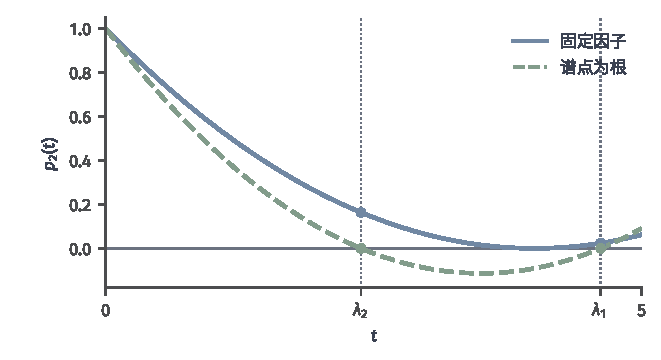
\includegraphics{figures/02-vectors-matrices-and-multivariate-calculus/03-linear-equations-and-optimization/matplotlib/learning-mechanisms/krylov-polynomial-roots.pdf}
  \caption{贯穿例$\bm A=\left[\begin{smallmatrix}4&1\\1&3\end{smallmatrix}\right]$的残差多项式。蓝线为Richardson两步的$(1-t/4)^2$，绿虚线为$1-7t/11+t^2/11$；圆点标记两个特征值处的值。二者均满足$p_2(0)=1$，只有后者在两个谱点同时为零。这是解释多项式自由度的解析对照，实际算法不需要预先知道特征值。}
  \label{fig:solver-krylov-polynomial-roots}
\end{figure}

\paragraph{选择策略}
实际计算中不知道特征值，不能像上例那样直接写出根。各方法改用可以计算的准则，在$\mathcal P_k$中隐式地选出$p_k$。准则所衡量的对象有两个。

一个是\emph{误差}
\begin{equation}
 \bm e_k=\bm x_k-\bm x_\star=p_k(\bm A)\bm e_0 ,
 \label{eq:ls-krylov-error-polynomial}
\end{equation}
后一个等式由$\bm e_k=-\bm A^{-1}\bm r_k$及$\bm A^{-1}$与$p_k(\bm A)$可交换得到。

另一个是\emph{残差}
\[
 \bm r_k=\bm b-\bm A\bm x_k=p_k(\bm A)\bm r_0 ,
\]
它可以直接算出。

误差才是我们真正关心的量，但它含未知的$\bm x_\star$，一般无法直接计算。所以一般使用残差来替代对误差的估计。

按所衡量的对象，Krylov子空间方法分为四类。

\emph{第一类：使误差最小。}误差一般算不出来，只有$\bm A$对称正定时是例外。这时误差的能量范数满足
\begin{equation}
 \lVert\bm e_k\rVert_{\bm A}^2=\bm e_k^\top\bm A\bm e_k=\bm r_k^\top\bm A^{-1}\bm r_k ,
 \label{eq:ls-krylov-energy-norm-identity}
\end{equation}
即误差的能量范数等于残差在$\bm A^{-1}$下的长度，两者是同一个量。

把近似写成
\[
  \bm x_k=\bm x_0+\bm V_k\bm y ,
\]
$\bm V_k$的列是$\mathcal K_k$的一组基，上式是$\bm y$的凸二次函数，令其梯度为零，得
\begin{equation}
 \bm V_k^\top\bm A(\bm x_\star-\bm x_0-\bm V_k\bm y)=\bm V_k^\top(\bm r_0-\bm A\bm V_k\bm y)=\bm0 .
 \label{eq:ls-krylov-galerkin-condition}
\end{equation}
条件中只出现残差，不出现$\bm x_\star$。它要求残差与子空间$\mathcal K_k$正交，称为Galerkin条件。

所以在$\bm x_0+\mathcal K_k$中使误差的能量范数最小，不必知道$\bm x_\star$就能做到；所选的$p_k$使$\lVert p_k(\bm A)\bm e_0\rVert_{\bm A}$在$\mathcal P_k$中最小，同时也就使残差的$\bm A^{-1}$长度最小。共轭梯度法（第~\ref{sec:ls-conjugate-gradient}节）采用这一策略。它控制的是这两种加权长度，欧氏残差$\lVert\bm r_k\rVert_2$不必每步下降。

\emph{第二类：使残差最小。}没有对称正定性提供的保证时，一般直接要求残差的欧氏长度
\[
 \lVert\bm r_k\rVert_2=\lVert p_k(\bm A)\bm r_0\rVert_2
\]
在$\mathcal P_k$中最小。这只要求$\bm A$可逆，并且因$\mathcal K_k\subseteq\mathcal K_{k+1}$，残差长度随$k$单调不增。MINRES（第~\ref{sec:ls-minres}节）对对称矩阵、GMRES（第~\ref{sec:ls-gmres}节）对一般方阵采用这一策略；前者借对称性只用短递推，后者要保存全部基向量。

长方矩阵的最小二乘问题中，LSQR（第~\ref{sec:ls-lsqr}节）在$\mathcal K_k(\bm A^\top\bm A,\bm A^\top\bm b)$中使原残差$\lVert\bm b-\bm A\bm x_k\rVert_2$最小，残差多项式的变量换成$\bm A^\top\bm A$。

\emph{第三类：使正规残差最小。}不相容的最小二乘问题中，原残差不会趋于零，判断是否已到最小二乘解要看正规方程的残差$\bm A^\top(\bm b-\bm A\bm x_k)$。LSQR使原残差单调下降，但正规残差的长度在病态问题中可能有小幅波动，不便作为停止判据。LSMR（第~\ref{sec:ls-lsmr}节）在同一个子空间中改为使正规残差的长度$\lVert\bm A^\top(\bm b-\bm A\bm x_k)\rVert_2$最小，于是它随$k$单调不增。

\emph{第四类：由正交条件确定。}对非对称矩阵，第二类准则需要保存全部基向量。若希望像对称情形那样只用短递推，常规的残差无法给出三项递推，于是BiCG（第~\ref{sec:ls-bicg}节）另取一个向量$\widetilde{\bm r}_0$，称为\term{影子残差}（shadow residual），并生成$\bm A^\top$的Krylov子空间
\begin{equation}
 \mathcal L_k=\mathcal K_k(\bm A^\top,\widetilde{\bm r}_0)=\operatorname{span}\{\widetilde{\bm r}_0,\bm A^\top\widetilde{\bm r}_0,\ldots,(\bm A^\top)^{k-1}\widetilde{\bm r}_0\}.
 \label{eq:ls-krylov-test-space}
\end{equation}
它不再寻找使某个长度最小的$p_k$，而是规定残差必须与$\mathcal L_k$正交，这样的$\mathcal L_k$称为\term{检验空间}（test space）。设$\bm W_k$的列是$\mathcal L_k$的一组基，条件$\bm W_k^\top(\bm r_0-\bm A\bm V_k\bm y)=\bm0$就是$k$阶方程
\begin{equation}
 (\bm W_k^\top\bm A\bm V_k)\,\bm y=\bm W_k^\top\bm r_0 ,
 \label{eq:ls-krylov-projection}
\end{equation}
解出$\bm y$，就由代数关系唯一地确定了$p_k$。

检验空间与子空间不同的这类条件，统称为Petrov--Galerkin条件；第一类中的Galerkin条件是$\mathcal L_k=\mathcal K_k$的特例。这样选出的$p_k$不使任何长度最小，残差可能剧烈起伏，方程~\eqref{eq:ls-krylov-projection}的系数矩阵也可能奇异而使迭代中断。

BiCGSTAB（第~\ref{sec:ls-bicgstab}节）在BiCG的多项式上每步再乘一个一次因子$1-\omega_jt$，并按局部的残差极小化选取$\omega_j$，以减缓这种起伏。这里不展开这一条件的几何意义，只把它作为选择$p_k$的第四种方式。

综上，本章的方法按选择$p_k$的准则分为四类：使误差（能量范数）最小的CG，使残差最小的MINRES、GMRES与LSQR，使正规残差最小的LSMR，以及由与影子子空间正交确定$p_k$的BiCG与BiCGSTAB。
